Presentation layer is where the interaction between human and machine takes place. This layer is further divided into 3 subsystems that continuously interact with each other to successfully communicate with the user. The screen of a mobile device will help the user to explore the various features of the application. Request subsystem is involved in receiving the commands of the user, XML subsystem will receive the command from Request subsystem. This subsystem will help to decode the instructions and complete the task. The response subsystem will display the result after the command is executed.

\subsection{Request}
Request is a fundamental subsystem of the Presentation layer. This subsystem will help to process the user given command. The commands may vary; the variety includes, signing up for new account, logging in to an already existing account, add to item to inventory, delete items from inventory, and search the inventory.

\begin{figure}[h!]
	\centering
 	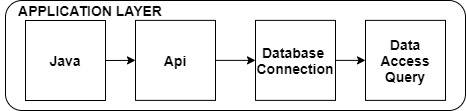
\includegraphics[width=0.60\textwidth]{images/App.jpg}
 \caption{Example subsystem description diagram}
\end{figure}

\subsubsection{Assumptions}
We assume that all the data entered by the user are accurate and valid for the application layer to process.

\subsubsection{Responsibilities}
This subsystem will be responsible to process the instructions entered by the user to the application layer. 

\subsubsection{Subsystem Interfaces}
Each of the inputs and outputs for the subsystem are defined here. Create a table with an entry for each labelled interface that connects to this subsystem. For each entry, describe any incoming and outgoing data elements will pass through this interface.

\begin {table}[H]
\caption {Subsystem interfaces} 
\begin{center}
    \begin{tabular}{ | p{1cm} | p{6cm} | p{3cm} | p{3cm} |}
    \hline
    ID & Description & Inputs & Outputs \\ \hline
    \#1 & The request subsystem will interact with the user to understand what the wants from the application. This will include SignUp, Login, store information or retrieve information from database & Email ID, User name, password, Age, First Name and Last Name & Registered or denied \\ \hline
    \#2 & The request subsystem will interact with the user to understand what the wants from the application. This will include Login. & \pbox{username, password} & \pbox{login success or denied due to incorrect credentials}  \\ \hline
    \end{tabular}
\end{center}
\end{table}

\subsection{XML}
XML is the unseen mechanics of our Presentation layer. The layouts, images or buttons seen in the application are functional because of XML. There are various kinds of XML files. Manifest XML file will help to define the functionality of buttons, layout XML file will help to determine the layout and many more XML files are available to help make the user-system interaction easy. 

\begin{figure}[h!]
	\centering
 	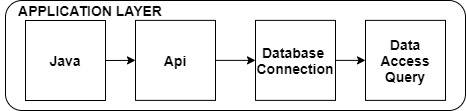
\includegraphics[width=0.60\textwidth]{images/App.jpg}
 \caption{Example subsystem description diagram}
\end{figure}

\subsubsection{Assumptions}
The user will issue right commands.

\subsubsection{Responsibilities}
The main responsibility of this subsystem is to form a connection with application layer from the presentation layer depending on what the user wants to do.

\subsubsection{Subsystem Interfaces}
Each of the inputs and outputs for the subsystem are defined here. Create a table with an entry for each labelled interface that connects to this subsystem. For each entry, describe any incoming and outgoing data elements will pass through this interface.

\begin {table}[H]
\caption {Subsystem interfaces} 
\begin{center}
    \begin{tabular}{ | p{1cm} | p{6cm} | p{3cm} | p{3cm} |}
    \hline
    ID & Description & Inputs & Outputs \\ \hline
    \#1 & User wants to search for an item(s) already in the inventory & Items to search by name, expiry date, flavor & Lists of product that match the search criteria.  \\ \hline
    \end{tabular}
\end{center}
\end{table}

\subsection{Response}
This subsystem is essential in order to successfully display the output that is asked by the user. The information gained from the request layer is processed by the application layer using database access layer if necessary in order to produce the desired out for the response subsystem.

\begin{figure}[h!]
	\centering
 	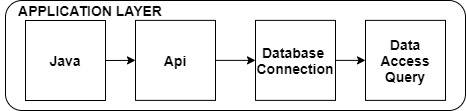
\includegraphics[width=0.60\textwidth]{images/App.jpg}
 \caption{Example subsystem description diagram}
\end{figure}

\subsubsection{Assumptions}
We assume that the query made by user can be successfully executed by application layer.

\subsubsection{Responsibilities}
This subsystem is responsible to display the result that is required from the users query.

\subsubsection{Subsystem Interfaces}
Each of the inputs and outputs for the subsystem are defined here. Create a table with an entry for each labelled interface that connects to this subsystem. For each entry, describe any incoming and outgoing data elements will pass through this interface.

\begin {table}[H]
\caption {Subsystem interfaces} 
\begin{center}
    \begin{tabular}{ | p{1cm} | p{6cm} | p{3cm} | p{3cm} |}
    \hline
    ID & Description & Inputs & Outputs \\ \hline
    \#1 & The user wants to look in to inventory for a certain product.  & Name of the product or search by specific requirement. & Detailed description of the product.  \\ \hline
    \end{tabular}
\end{center}
\end{table}
